\documentclass{article}
\usepackage[utf8]{inputenc}
\usepackage{graphicx}
\usepackage{amsmath}
\usepackage{amsfonts}
\usepackage{geometry}
\usepackage{hyperref}

\geometry{a4paper, margin=1in}

\title{Reconnaissance de chiffres manuscrits par plus proches voisins}
\author{Joris Lasserre}
\date{}

\begin{document}

\maketitle

\section{Introduction}

\subsection{Présentation du projet}
L'objectif de ce projet est de développer une application de reconnaissance de chiffres manuscrits. Le principe est simple, fournir un chiffre manuscrit au programme sans préciser son intitulé, et le programme doit être capable de l'identifier. Pour cela, nous utiliserons l'apprentissage supervisé. Selon la définition de la CNIL, ``l'apprentissage supervisé est un procédé d'apprentissage automatique dans lequel l'algorithme s'entraîne à une tâche déterminée en utilisant un jeu de données assorti de chaque annotation indiquant le résultat attendu.'' 

Nous nous appuierons plus particulièrement sur l'algorithme des k-plus proches voisins (k-Nearest Neighbors ou k-NN) dans ce projet. L'algorithme K-NN va permettre de trouver le résultat en analysant les distances calculées entre nos nombres et en prenant comme réponse l'intitulé le plus fréquent parmi les K voisins les plus proches. Maintenant que nous avons vu l'objectif du projet, nous allons pouvoir nous pencher en détail sur la base de données utilisée et les enjeux scientifiques de celui-ci. 

\subsection{Présentation de la base}
La base de données utilisée est un extrait de 120 images, 10 de chaque chiffre et caractère ``plus'' et ``moins'', issus de la base de données du MNIST (Modified National Institute of Standards and Technology database). J'ai décidé par gain de temps de ne pas traiter les signes ``plus'' et ``moins''. 

Ces images sont toutes ``labélisées'' par l'intitulé de leur chiffre, ce qui nous permettra plus tard de comparer la prédiction de notre programme avec les résultats attendus. Un point important à uniformiser lors de la partie traitement d'image est le fait que les images n'aient pas toutes la même taille, ce qui pourrait poser problème. 

\subsection{Les enjeux scientifiques de la reconnaissance de caractères}
À première vue, nous pourrions penser qu'une application qui reconnaît des nombres manuscrits n'a d'utilité que celle de divertir un groupe d'étudiants en informatique. Néanmoins, lorsqu'on y réfléchit un peu plus, on y trouve de nombreuses utilités, comme le traitement de documents (chèques, numérisation de dossiers), la reconstitution de papyrus altérés par le temps, ou encore la détection des inscriptions écrites sur les panneaux routiers utilisée par les voitures autonomes.

Nous pouvons même évoquer le fait que la reconnaissance de caractères manuscrits permet d'alimenter d'autres IA ou algorithmes capables d'imiter l'écriture manuscrite humaine à partir de seulement quelques images, comme le réseau ``GANwriting''. À terme, l'objectif serait d'avoir des modèles généraux capables de reconnaître la quasi-totalité des langues, malgré le bruit, notamment celles avec des alphabets différents ou des styles d'écriture particuliers et difficiles à lire, comme l'écriture cursive russe. 

Enfin, la reconnaissance de caractères manuscrits n'est qu'un premier pas dans les sciences de la reconnaissance d'image. En effet, ces techniques sont ou seront déjà utilisées dans divers domaines allant de la médecine à l'automobile, en passant par l'archéologie. 

\section{Proposition d’une solution}

\subsection{Chaîne de traitement et d'analyse}
La chaîne de traitement que j'ai mise en place comporte quatre parties. Pour illustrer le processus, je vais modifier le chiffre ci-dessous dont voici l'image originale : 

\begin{figure}[h!]
    \centering
    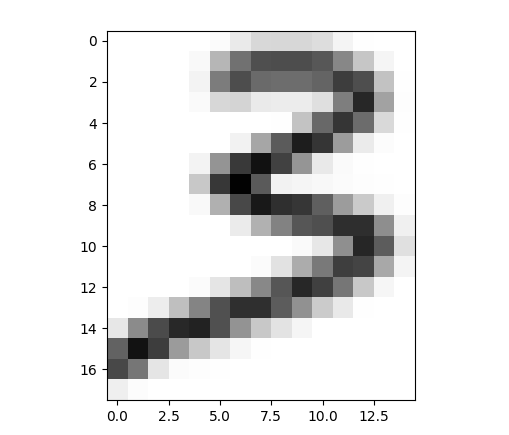
\includegraphics[width=0.5\textwidth]{images/original_picture.png}
\end{figure}

Étant donné que les images n'ont pas toutes la même taille, la première étape consiste à les redimensionner pour les uniformiser.

\begin{figure}[h!]
    \centering
    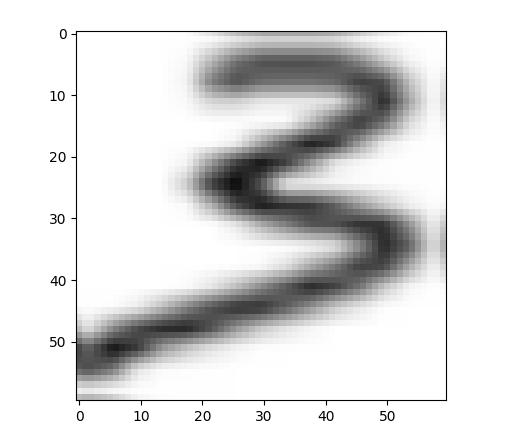
\includegraphics[width=0.5\textwidth]{images/resized_picture.png}
\end{figure}

Ensuite pour pouvoir appliquer l'érosion, la dilatation et faciliter le comptage des pixels il est nécessaire de binariser l'image. C'est à dire convertir chaque pixel en noir ou en blanc. Une étape intermédiaire consiste d'abord à convertir l'image en niveaux de gris. 

\begin{figure}[h!]
    \centering
    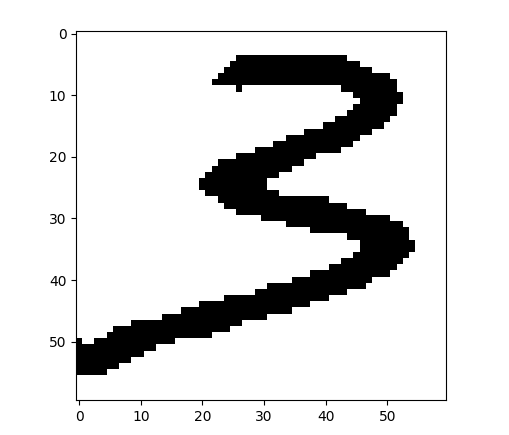
\includegraphics[width=0.5\textwidth]{images/binarised_picture.png}
\end{figure}

Une fois cette étape terminée, nous appliquons une érosion pour éliminer les zones de bruit et autres formes susceptibles d'altérer la reconnaissance.

\begin{figure}[h!]
    \centering
    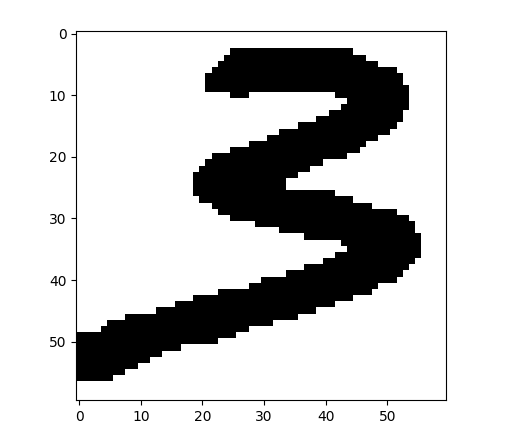
\includegraphics[width=0.5\textwidth]{images/eroded_picture.png}
\end{figure}

Enfin, nous procédons à une dilatation pour restaurer la qualité de certains chiffres.

\begin{figure}[h!]
    \centering
    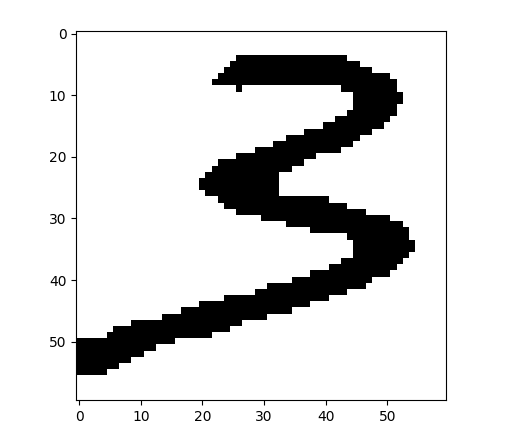
\includegraphics[width=0.5\textwidth]{images/dilatation_picture.png}
\end{figure}

Dans ce cas particulier, l'image binarisée et l'image finale semblent similaires. Cependant, sur l'ensemble des images, ces étapes permettent de gagner en précision en éliminant certains bruits et en se concentrant sur les traits caractéristiques du chiffre.

\subsection{Détail d’un algorithme d’extraction de caractéristiques}
J'ai choisi d'utiliser comme algorithme d'extraction de caractéristiques le ``Zoning''. Celui-ci consiste à découper l'image binarisée en blocs et à calculer pour chaque bloc une caractéristique précise. Dans notre cas cette caractéristiques est le nombre de pixel noir. 

Dans la manière dont j'ai implémenté l'algorithme, je ne spécifie pas directement le nombre de blocs souhaité pour la découpe de l'image. A la place je prends le carré de N. Dans mon cas, comme N vaut 5, mes images sont divisées en 25 blocs. L'algorithme retourne à la fin un vecteur de N caractéristiques. 

Exemple de vecteur de caractéristiques pour un chiffre 3 : [0, 3, 58, 65, 21, 0, 6, 55, 62, 13, 0, 12, 69, 68, 34, 3, 33, 58, 63, 18, 69, 27, 1, 0, 0].

\section{Analyse des résultats}
Pour rappel, l'objectif de notre programme est de reconnaître des chiffres manuscrits allant de 0 à 9. Pour évaluer les performances de l'algorithme, nous avons effectué 100 tests avec les critères suivants : 

\begin{itemize}
    \item 99 images sont utilisées comme base d'apprentissage.
    \item L'image restante sert de test, et son label n'est pas connu à l'avance.
    \item Nous calculons la distance entre le vecteur représentant l'image de test et ceux des 99 autres images.
    \item Les distances sont triées par ordre croissant.
    \item Les K plus petites distances sont sélectionnées (Dans mon cas, k = 3).
    \item Le label le plus présent parmi les K voisins les plus proches est attribué à l'image de test.
    \item Si la prédiction est correcte, nous incrémentons le nombre de bonnes réponses.
    \item Le pourcentage de bonnes réponses est calculé à partir du nombre de prédictions correctes sur le nombre total de réponse puis multiplié par 100.
\end{itemize}

\subsection{Présentation d’une matrice de confusion}
Avant de vous montrer le résultat final sous forme de matrice de confusion, je vais vous en expliquer le fonctionnement.

Une matrice de confusion est un tableau 2D où les lignes représentent les labels réels et les colonnes les labels prédits. Les valeurs sur la diagonale indiquent les prédictions correctes, tandis que les valeurs hors diagonale représentent les erreurs. Dans notre cas, le programme sait reconnaître un nombre lorsque le chiffre dans la diagonale est 10/10. 

\begin{figure}[h]
    \centering
    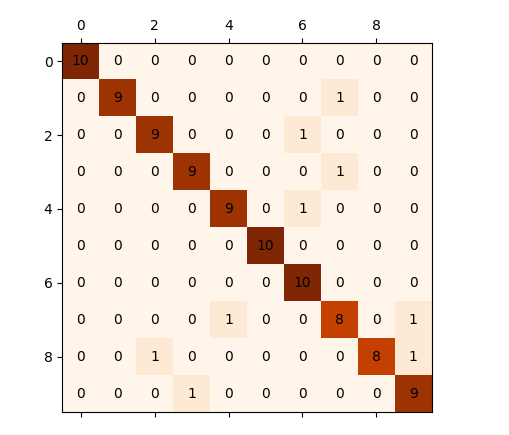
\includegraphics[width=0.5\textwidth]{images/matrice_confusion.png}
\end{figure}

Le résultat final que j'obtiens est cette matrice de confusion avec un taux de reconnaissance de 91\%. Les paramètres qui parviennent à avoir ce taux de réussite sont : 
\begin{itemize}
    \item nombre de plus k-proches voisins considérés : 3
    \item Nombre de blocs : 25.
    \item Taille de l'élément structurant pour l'érosion et la dilatation : 3.
    \item Dimensions de redimensionnement : 60x60 pixels.
\end{itemize}

\subsection{Analyse des erreurs}
Nous allons essayé de comprendre les cas où le programme n'a pas donné la bonne réponse. 

L'une des premières erreurs est la confusion "naturelle" entre le 7 et le 1, en raison de leur ressemblance lorsqu'ils sont écrits à la main.

On remarque aussi, des erreurs pour le chiffre 8. Les traitements appliqués aux images altèrent parfois la forme des 8, les rendant similaires à d'autres chiffres, comme le 9. 

\begin{figure}[h]
    \centering
    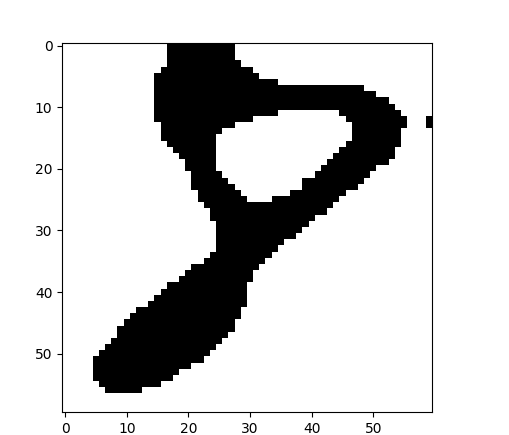
\includegraphics[width=0.5\textwidth]{images/8_similaire_9.png}
\end{figure}

Je pense que ces "malformations" sont le cas le plus courant de mes erreurs, elles modifient certains autres chiffres déjà mal écrit ce qui entraîne une mauvaise estimation. 
Néanmoins certaines erreurs restent mystérieuses et nécessisteraient d'approfondir plus les recherches comme pourquoi un 4 a été estimé un 6. 

\section{Conclusion}
En conclusion, nous avons développé un programme de reconnaissance de chiffres manuscrits avec un taux de réussite de 91\%. Ce résultat peut être amélioré en augmentant le nombre de données d'entraînement, en incluant davantage de cas pouvant porter à confusion. Il serait également possible d'affiner les étapes de dilatation et d'érosion pour éliminer le bruit tout en conservant les formes des chiffres.

\end{document}
